%%\documentclass[final,3p,times,twocolumn]{elsarticle}
\documentclass[final,3p]{book}

%\includeonly{cs}

%% Use the option review to obtain double line spacing
%% \documentclass[preprint,review,12pt]{elsarticle}

%% Use the options 1p,twocolumn; 3p; 3p,twocolumn; 5p; or 5p,twocolumn
%% for a journal layout:
%% \documentclass[final,1p,times]{elsarticle}
%% \documentclass[final,1p,times,twocolumn]{elsarticle}
%% \documentclass[final,3p,times]{elsarticle}
%% \documentclass[final,3p,times,twocolumn]{elsarticle}
%% \documentclass[final,5p,times]{elsarticle}
%% \documentclass[final,5p,times,twocolumn]{elsarticle}

%% if you use PostScript figures in your article
%% use the graphics package for simple commands
%% \usepackage{graphics}
%% or use the graphicx package for more complicated commands
%% \usepackage{graphicx}
%% or use the epsfig package if you prefer to use the old commands
%% \usepackage{epsfig}

%% The amssymb package provides various useful mathematical symbols
\usepackage{amssymb}
%% The amsthm package provides extended theorem environments
%% \usepackage{amsthm}
%% The bm package lets you access bold symbols in math mode using the \boldsymbol command (useful to get bold greek letters).
\usepackage{bm}
%% The bbm package is contains the indicator function symbol \mathbbm{1}
\usepackage{bbm}
%% The amsmath package contains the split environment, letting you split equations into multiple lines.
%% See "https://www.sharelatex.com/learn/Aligning_equations_with_amsmath " for an explanation.
\usepackage{amsmath}
%% The lineno packages adds line numbers. Start line numbering with
%% \begin{linenumbers}, end it with \end{linenumbers}. Or switch it on
%% for the whole article with \linenumbers after \end{frontmatter}.
%% \usepackage{lineno}
%% The algorithm defines the algorithm floating environment and the algpseudocode package is useful for constructing Pseudo code.
\usepackage{algorithm}
\usepackage{algpseudocode}
%% For creating pictures
\usepackage{tikz}
%% For making algorithms float
\usepackage{float}
\newfloat{algorithm}{t}{lop}
%% For creating draft watermark
%\usepackage{draftwatermark}
%\SetWatermarkText{DRAFT}
%\SetWatermarkScale{1}
\usepackage{pdfpages}

%% Declaring \argmin and \argmax operators:
\DeclareMathOperator*{\argmin}{arg\,min}
\DeclareMathOperator*{\argmax}{arg\,max}
%% Declare trace operator \Tr:
\DeclareMathOperator*{\Tr}{Tr}
%% Declare pdf functions
\DeclareMathOperator*{\Cat}{Cat}
\DeclareMathOperator*{\Dir}{Dir}
\DeclareMathOperator*{\DP}{DP}
\DeclareMathOperator*{\Beta}{Beta}
\DeclareMathOperator*{\GEM}{GEM}
\DeclareMathOperator*{\Stick}{Stick}
\DeclareMathOperator*{\Uniform}{Uniform}
%% shorthand for \boldsymbol and \overline
\let\bs\boldsymbol
\let\ol\overline
%% command that allows equations to be split across pages
%\allowdisplaybreaks[3]

%% natbib.sty is loaded by default. However, natbib options can be
%% provided with \biboptions{...} command. Following options are
%% valid:

%%   round  -  round parentheses are used (default)
%%   square -  square brackets are used   [option]
%%   curly  -  curly braces are used      {option}
%%   angle  -  angle brackets are used    <option>
%%   semicolon  -  multiple citations separated by semi-colon
%%   colon  - same as semicolon, an earlier confusion
%%   comma  -  separated by comma
%%   numbers-  selects numerical citations
%%   super  -  numerical citations as superscripts
%%   sort   -  sorts multiple citations according to order in ref. list
%%   sort&compress   -  like sort, but also compresses numerical citations
%%   compress - compresses without sorting
%%
%% \biboptions{comma,round}

% \biboptions{}


%\journal{MPhil in Scientific Computing}

\begin{document}

%% for elsarticle class
\begin{frontmatter}

%% Title, authors and addresses

%% use the tnoteref command within \title for footnotes;
%% use the tnotetext command for the associated footnote;
%% use the fnref command within \author or \address for footnotes;
%% use the fntext command for the associated footnote;
%% use the corref command within \author for corresponding author footnotes;
%% use the cortext command for the associated footnote;
%% use the ead command for the email address,
%% and the form \ead[url] for the home page:
%%
%% \title{Title\tnoteref{label1}}
%% \tnotetext[label1]{}
%% \author{Name\corref{cor1}\fnref{label2}}
%% \ead{email address}
%% \ead[url]{home page}
%% \fntext[label2]{}
%% \cortext[cor1]{}
%% \address{Address\fnref{label3}}
%% \fntext[label3]{}

\begin{titlepage}
\begin{center}
\includegraphics[width=0.6\textwidth]{Images/cam.png}\\

\vspace*{4cm}
\Huge\textbf{Compressive Sensing in Video Reconstruction}

\vspace*{1.5cm}
\LARGE
\textbf{Brian Azizi}
\vfill

\normalsize
A thesis submitted in partial fulfillment of the requirements for\\
the degree of Master of Philosophy

\vspace{0.8cm}

\normalsize
Supervised by:\\
Dr Anita Faul

\vspace{0.2cm}
Department of Physics\\
Cavendish Laboratory\\
JJ Thomson Avenue\\
CB3 0HE\\
Cambridge, UK\\
\vspace{0.4cm}
\normalsize
\today

\end{center}
\end{titlepage}



\title{Compressive Sensing in Video Reconstruction}

%% use optional labels to link authors explicitly to addresses:
%% \author[label1,label2]{<author name>}
%% \address[label1]{<address>}
%% \address[label2]{<address>}

\author{Brian Azizi}

%\address{Cavendish Laboratory, Department of Physics, J J Thomson
 % Avenue, Cambridge. CB3 0HE}


\tableofcontents

\end{frontmatter}

%%
%% Start line numbering here if you want
%%
% \linenumbers

%% main text
\chapter{Introduction}

There are three parts: A signal processing framework called \emph{Compressive Sensing (CS)}, a pre-processing step in form of a basis transformation based on discrete wavelet transforms and a Machine Learning algorithm called \emph{Sparse Bayesian Learning}.

The key notion that ties in these three areas is the notion of \emph{sparsity}.

\section*{Background}


\chapter{Compressive Sensing}
\label{ch:cs}

% \emph{
% \begin{itemize}
% \item Problem Statement for discrete. Img, Vids as unrolled vec. Sparsity -> Compression (adaptive). Why wasteful.
% \item CS is NON-ADAPTIVE. Sensing Matrix. Much fewer measurements.
% \item Against Fund Thm of LA -> resolve by sparsity (show a graphic).
% \item What Sensing matrix? We've only done masks, so maybe no point in talking about RIP etc -> just reference.
% \item Signal Recovery. L2 vs L0 vs L1 + Geometry?.
% \item We focus on Reconstruction. Side note to single-px cam (in \@ sensing). Perhaps this should go in Ch1:Background
% \item Bayesian CS (or put it in Ch5?)
% \end{itemize}
% }

% \emph{
%   \begin{enumerate}
%   \item Conventional DSP + Promise of CS
%   \item CS Problem
%   \item CS Solution Strategy
%     \begin{enumerate}
%     \item Sparsity
%     \item Incoherence
%     \end{enumerate}
%   \item CS Reconstruction
%   \end{enumerate}
% }


In this chapter we will outline the main ideas of the \emph{Compressive Sensing} framework (also known as \emph{Compressed Sensing, Compressed Sampling, Compressive Samping} or \emph{CS}).
We begin by discussing conventional approaches to data acquisition and compression, and how CS differs from that.
Next, formulate the CS Problem.
Following that, we briefly discuss the general solution strategy.
Lastly, give a brief overview of deterministic approaches to CS reconstruction (maybe).

In Chapter \ref{ch:msce}, we will discuss a Bayesian approach to solving the Compressive Sensing Problem.


\section{Signal Acquisition and Compression}
\subsection{Acquisition}
In order to work with information within analog signals (continuous streams of data) such as sounds, images or video, we rely on reducing the analog signals to digital (discrete) signals that can be processed with computers.
This digitization is done by taking discrete measurements of the analog signal at certain points in time or space, a process known as \emph{sampling}.

Conventional approaches to sampling are based on the \emph{Shannon/Nyquist Sampling Theorem} \cite{shannon1949}:
When sampling a band-limited signal uniformly, we are able to \emph{perfectly reconstruct} the signal from its samples if the sampling rate is at least twice the bandwidth of the signal.

We briefly illustrate this in Figure \ref{fig:nyquist}.
Consider an analog signal $x(t)$ that varies with time, such as an audio wave.
Let $f$ be the highest frequency present in $x(t)$.

In order to digitise $x(t)$, we measure $x$ at discrete points in time $t^{(0)}, \cdots, t^{(n)}$ and store the samples $x^{(i)} \equiv x(t^{(i)})$.
We sample $x$ uniformly, measuring a sample every $T_s$ seconds, so that $t^{(i)} = iT_s$.
The sampling rate is therefore $f_s = 1/T_s$.

\begin{figure}
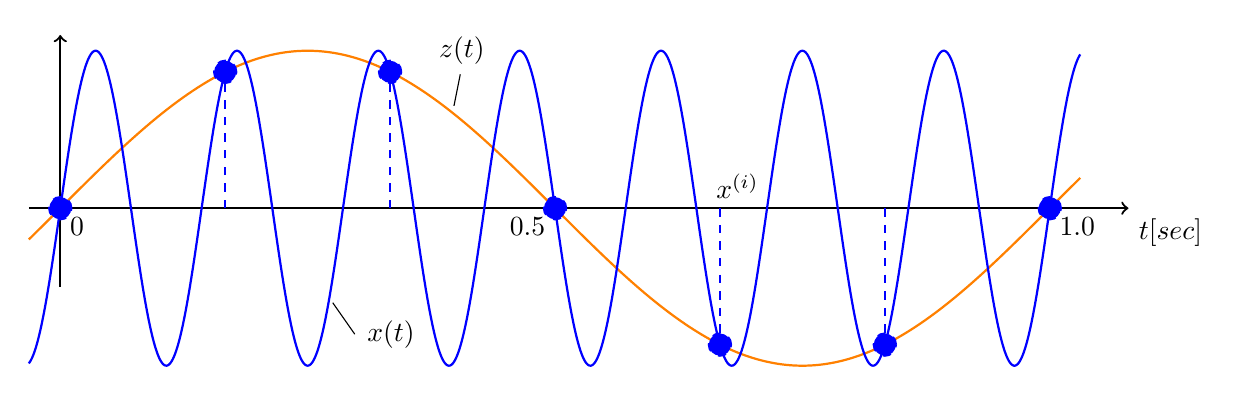
\begin{tikzpicture}[scale=2]
  \draw [thick,->](-0.2,0) -- (2*pi+0.5,0) node[below right] {$t [sec]$};
  \draw [thick,->](0,-0.5) -- (0,1.1);
  \draw [domain=-0.2:2*pi+0.2,samples=1000,orange, thick] plot(\x,{sin(\x r)});
  \draw [domain=-0.2:2*pi+0.2,samples=1000,blue, thick] plot(\x,{sin(7*\x r)});  
  \draw [domain=0:2*pi, samples=7, ycomb, mark=*,blue, dashed, thick] plot(\x,{sin(\x r)});
  \node at (2.55,1) {$z(t)$};
  \draw (2.54,0.85) -- (2.5,0.65);
  \node at (2.1,-0.8) {$x(t)$};
  \draw (1.87,-0.8) -- (1.73,-0.6);
  \node at (4.3,0) [above] {$x^{(i)}$};
  \node at (2*pi,0) [below right] {$1.0$};
  \node at (pi,0) [below left] {$0.5$};
  \node at (0,0) [below right] {$0$};
\end{tikzpicture}
\caption[Illustration of Nyquist Sampling]{Illustration of the Shannon/Nyquist Sampling Theorem. The orange curve is the original signal $x(t)$ which is a sinusoid with frequency $f = 7$ Hz. The blue points are discrete samples $x^{(i)}$ taken from $x(t)$ at a sampling rate $f_s = 7$ Hz, which is below the Nyquist Rate $2f = 14$ Hz. Thus, aliasing occurs and interpolation algorithms will reconstruct an alias $z(t)$ of $x(t)$.}
\label{fig:nyquist}
\end{figure}

Suppose we wish to reconstruct $x(t)$ by interpolating the samples.
There is an infinite number of continuous functions that fit this set of samples.
However, it can be shown that only one of them has a bandwidth of no more than $f_s/2$.
Thus, if $f < f_s/2$ (the \emph{Nyquist Criterion}), then $x(t)$ is the unique function that will be approximated by interpolation algorithm such as the \emph{Whittaker-Shannon interpolation formula}\cite{shannon1949}.

In Figure \ref{fig:nyquist}, we have a sinusoidal signal $x(t)$ with frequency $f$.
The sampling rate is $f_s=f$ and therefore below the signal's \emph{Nyquist rate} $2f$. 
Thus, we are unable to reconstruct $x(t)$ from the samples. 
Instead, we will reconstruct an \emph{alias} $z(t)$ which, in this case, is another sinusoid with frequency $f/7$.
The original signal $x$ is lost.

We have illustrated Nyquist sampling in the 1-dimensional case.
The same principles hold for higher dimensional signals such as images and videos.

For signals that vary with space, the sampling rate is governed by the desired spatial resolution.
In order to recover the finer details (the high-frequency components) of an image, we require higher pixel density (i.e. more pixels per 

Nyquist sampling underlies almost all signal acquisition protocols that are found in practice. 
It is the basis of medical imaging devices, consumer electronics such as audio and video recorders, radio receivers, etc.

\subsection{Compression}
The sampling theorem imposes a lower bound on the sampling rate above which we get are able to perfectly reconstruct the desired signal.
This lower bound is often very high and we end up with a very large number of measurements.
Storage and transfer of such signals becomes prohibitavely expensive as the size of the signal grows.
Thus, a need for \emph{data compression} arises.

We will discuss a particular type data compression known as \emph{transform coding}.
It is the standard compression method for ``natural'' and manmade signals such as audio, photos, and video and is the basis of many common signal formats such as JPEG for images, MPEG for videos and MP3 for audio.

Let $\bm v$ by a real-valued digital signal of length $M$, $\bm v \in \mathbb{R}^M$.
Without loss of generality, $\bm v$ is assumed to be a one-dimensional signals.
If we are working with a multi-dimensional signals, we may first vectorize it into a long vector.
When compressing digital signals, we are usually interested in \emph{lossy compression}.

Any vector in $\mathbb{R}^M$ can be expressed as a linear combination of $M$ \emph{basis vectors} $\bm\psi_j \in \mathbb{R}^M$:
\begin{equation}
\label{eqn:cs-transform1}
  \bm v = \sum_{j=1}^M w_j \bm\psi_j
\end{equation}
where $w_j$ is the coefficient (or weight) associated with $\bm\psi_j$.

By forming the \emph{basis matrix} $\bm\Psi = \left[\bm\psi_1 \,\cdots\, \bm\psi_M\right]$, we can express equation (\ref{eqn:cs-transform1}) in matrix form
\begin{equation*}
\bm v = \bm\Psi \bm w
\end{equation*}
where $\bm w = (w_1,\cdots,w_M)^T$.
For simplicity, we assume that the basis $\bm\Psi$ is orthonormal, so that $\bm\Psi\bm\Psi^T = \bm I_M$ and $\bm\psi_i^T\bm\psi_j$ is 1 if $i = j$ and 0 otherwise.
Thus, the coefficient $w_j$ is given by $w_j = \bm v^T\bm\psi_j$.

We now have two equivalent representations of the same signal, $\bm v$ in the original basis and $\bm w$ in the $\bm\Psi$ basis.
Since $\bm\Psi$ is orthogonal, $\bm v$ and $\bm w$ have the same $\ell_2$-norm, $||\bm v||_2 = ||\bm\Psi\bm w||_2 = ||\bm w||_2$.

While in the original signal $\bm v$ the energy is spread over many of its components, it is possible to find a basis $\bm\Psi$ such that the energy of the transformed signal $\bm w$ is concentrated in only a few large components $w_j$.
Thus a large fraction of the entries in $\bm w$ are very close to zero.

Suppose that we delete the entries $w_j$ that are very small and replace them with zero to obtain $\bm{\hat w}$.
Let $\bm{\hat v} = \bm\Psi\hat{\bm w}$ the approximate signal in the original domain.
Since $\bm{\hat w}$ is very close to $\bm w$, so that $||\bm{\hat w} - \bm w||_2$ is very small, it follows that
\begin{equation*}
  ||\bm{\hat v} - \bm v||_2 = ||\Psi\bm{\hat w} - \Psi\bm w||_2 = ||\Psi (\bm{\hat w} - \bm w||_2 = ||\bm{\hat w} - \bm w)||_2
\end{equation*}
is also very small.

\begin{figure}
  \centering
  \begin{subfigure}[b]{0.4\textwidth}
    \includegraphics[width=\textwidth]{Chapter2/Images/lenna512.png}
    \caption{Uncompressed Image}
    \label{fig:ch2:lenna_orig}
  \end{subfigure}
  \begin{subfigure}[b]{0.4\textwidth}
    \includegraphics[width=\textwidth]{Chapter2/Images/lenna512_dct.png}
    \caption{Compressed Image via DCT}
    \label{fig:ch2:lenna_dct}
  \end{subfigure}
  \caption[Image Compression using DCT]{The uncompressed image has a resolution of $512\times 512$, i.e. 262144 pixels. We compress the image by performing a Discrete Cosine Transform and storing only the largest 27832 coefficients. The compression ratio is 9.42.}
  \label{fig:ch2:dct}
\end{figure}

Thus, a viable method for lossy compression of the signal $\bm v \in \mathbb{R}^M$ would be the following:
\begin{enumerate}
\item Compute the full set of transform coefficients $\{w_j\}_{j=1}^M$ via $\bm w = \Psi^T\bm v$.
\item Locate all the coefficients $w_j$ whose absolute value is above a certain threshold (suppose there are $K$ of them). 
\item Discard all the $(M-K)$ small coefficients
\item Store the values and locations of the $K$ large coefficients
\end{enumerate}
It is possible to find basis matrices $\bm\Psi$ that result in very high compression ratios for a wide range of natural signals without any noticable reduction in the signal quality.
Furthermore, many of the commonly used basis transforms can be computed very efficiently.

Audio signals and a wide class of communication signals are highly compressible in the localized Fourier basis.
Images and video signals are often compressed via the \emph{Discrete Cosine Transform} (DCT) or the \emph{Discrete Wavelet Transform} (DWT).
For instance, the JPEG standard for image compression is based on the DCT, while the more modern JPEG2000 format uses the CDF 9/7 wavelet transform or the CDF 5/3 wavelet transform \cite{taubman2012}.

In Figure \ref{fig:ch2:dct}, we compress the standard test image ``Lenna'' via a DCT. 
We are only storing about 10\% of the transform coefficients.
Yet, the difference between the original image and the compressed image is hardly noticable.

We will discuss the DCT and the DWT in more detail in Chapter \ref{ch:dwt}.

\subsection{A Novel Approach: Compressed Sampling}
Circumvent Shannon by non-uniform sampling or by using alternative sampling matrices.


\section{The Compressive Sensing Problem}



This section is based on \cite{pilikos2014}. 
The problem to be solved can be formulated as follows: Let $\bs x \in \mathbb{R}^N$ be a signal of interest.
We do not measure $\bs x$ directly and it is thus unknown.
Instead, we have a measurement $\bs y \in \mathbb{R}^M$, with $M << N$, from which we want to reconstruct $\bs x$.
The signals $\bs x$ and $\bs y$ are related as follows:
\begin{equation}
\label{eqn:CS}
\bs \Omega \bs x = \bs y
\end{equation}
where $\bs \Omega$ is a known $M\times N$ matrix referred to as the \emph{sensing matrix}.

For example, in \cite{pilikos2014}, the signal of interest $\bs x$ is an image, so that $N$ is equal to the total number of pixels in the image and $x_i$ is equal to the intensity of the corresponding pixel.
However, we imagine that we have only access to a corrupted version of $\bs x$ in which random pixel values have been deleted.
This is our measurement $\bs y$.
The sensing matrix $\bs\Omega$ corresponding to this scenario is obtained by taking the $N\times N$ identity matrix and deleting the rows that correspond to the missing entries in $\bs x$.

Compressive Sensing (CS) is a collection of signal processing techniques that allow for efficient \emph{reconstruction} (and indeed \emph{aquisition}) of such signals by solving the underdetermined system (\ref{eqn:CS}).

Of course, there are infinitely many solutions to an underdetermined system.
In the CS framework, we seek to find a solution $\hat{\bs x}$ that is \emph{sparsest in some domain}.
By that, we mean that we want to find $\hat{\bs x}$ that satisfies (\ref{eqn:CS}), such that there exists a basis transformation of $\hat{\bs x}$ in which it has the smallest number of nonzero entries.

More concretely, we assume there exists a domain in which the desired signal $\bs x$ is sparse. 
I.e. there exists a $N\times N$ basis matrix $\Psi$ such that $\bs x = \bs\Psi \bs w$ and $\bs w$ is sparse.

The CS problem can then be expressed as follows:
\begin{equation}
\label{eqn:CSproblem}
\min||\bs w||_0 \qquad\mbox{subject to}\qquad \bs\Omega\bs\Psi\bs w = \bs y
\end{equation}
where $||.||$ denotes the $l_0$ norm, i.e. the number of nonzero components.


\section{The Solution}
\subsection{Stable Measurement Matrix}
\emph{Matrices}
\subsection{Reconstruction Algorithms}
\emph{L0, L1, L2, Deterministic, Geometry}

For a more detailed review of the CS framework, see \cite{candes2008}.



\chapter{Basis Functions}
\label{ch:dwt}

%\item Explain MSE, PSNR
In Section \ref{sect:compression}, we introduced transform coding.
We said that any discrete signal $\bm v \in \mathbb{R}^M$ can be expressed in a different basis via a basis transform:
\begin{equation*}
  \bm v = \bm\Psi\bm w
\end{equation*}
where $\bm\Psi$ is the $M\times M$ basis matrix and $\bm w \in\mathbb{R}^M$ is the representation of $\bm v$ in the $\bm\Psi$ basis.

The particular classes of signals $\bm v$ that we are interested in are digital images and digital video.
The aim of this chapter is to construct a basis matrix $\bm\Psi$ that gives us a (near-) sparse representation of a wide range of such signals $\bm v$.
Finding a set of basis functions $\bs\Psi$ that achieve such a transformation lies at the heart of many lossy compression techniques.

It is important to note here that the choice of basis functions $\bm \Psi$ typically has a significant effect on the performance of the reconstruction algorithms.

\section{Discrete Cosine Transform}
\label{sect:dct}
The first basis transform that we will use is the Discrete Cosine Transform (DCT), one of the most widely used transforms in signal processing.
It underlies JPEG image compression and is used in various video compression algorithms such as MJPEG, MPEG, H.261 and H.263 \cite{zeng2013}.
\footnote{A related transform, known as the \emph{Modified DCT} is used in many lossy audio compression formats such as MP3, AAC and Vorbis.}

A DCT decomposes a signal in terms of cosine functions with different frequencies.
Its extensive use in lossy compression algorithms is due to the DCT's \emph{energy compaction} properties.
The majority of a signal's energy is contained within relatively few coefficients - typically those corresponding to the lower frequency basis functions.

On a side note, the DCT comes in a various versions that have minor differences between them.
In the following, we will describe the most widely used version, known as the \emph{DCT-II}, as well as its inverse transform, the \emph{DCT-III}.
We will refer to them simply as ``the DCT'' and ``the Inverse DCT (IDCT)'', respectively.

\subsection{One-Dimensional DCT}
\begin{figure}
  \centering
  \begin{subfigure}{0.45\textwidth}
    \centering
    \includegraphics[width=\textwidth]{Chapter3/Images/cameraman.png}
    \caption{Original signal $\bm v$}
  \end{subfigure}
  \begin{subfigure}{0.45\textwidth}
    \centering
    \includegraphics[width=\textwidth]{Chapter3/Images/dctCoeff.png}
    \caption{DCT of $\bm v$}
  \end{subfigure}
  \caption[Two-dimensional DCT applied to a digital image]{Panel (a) shows the original signal $\bm v$, a 256$\times$256 grayscale image known as ``cameraman''. Panel (b) illustrates the 2-D DCT of $\bm v$. The brightness of a an element increases with the absolute value of the corresponding DCT coefficient. (The high-frequency coefficients have been enhanced to show more detail).}
  \label{fig:ch3:dct}
\end{figure}

Formally, the DCT $\bm w$ of a one-dimensional signal $\bm v$ of length $M$ is given by
\begin{equation}
  \label{eqn:dct_basis}
  w_k = c(k) \sum_{m=1}^{M} v_m \, \cos\left(\frac{\pi(2i-1)(k-1)}{2M}\right) \qquad k = 1,\cdots,M
\end{equation}
where
\begin{equation*}
  c(k) = \left\{\begin{array}{ll}
  \sqrt{\frac{1}{M}} & \qquad\mbox{if $k=1$}\\
  \sqrt{\frac{2}{M}} & \qquad\mbox{otherwise}\\
  \end{array}\right.
\end{equation*}
This transforms a signal $\bm v$ in the original domain (time or space) into its representation $\bm w$ in the DCT domain.

\begin{figure}
  \centering
  \includegraphics[width=0.5\textwidth]{Chapter3/Images/dct2functions.png}
  \caption[The 2-D DCT basis functions]{The 2-D DCT basis functions that are used by the DCT to decompose a $4\times 4$ image. 
    The spatial frequency increases towards the bottom right corner.}
  \label{fig:2D-DCT}
\end{figure}

Conversely, given a signal $\bm w$ in the DCT domain, we can transform it back to the orignal (time or space) domain via the IDCT defined by
\begin{equation}
  \label{eqn:idct}
  v_n = \sum_{k=1}^M c(k) w_k  \, \cos\left(\frac{\pi(2i-1)(k-1)}{2M}\right) \qquad n = 1,\cdots,M
\end{equation}

We can express equation (\ref{eqn:idct}) in the desired form $\bm v=\bm P\bm w$.
The entries of the basis matrix $\bm P$ are given by
\begin{equation}
  \label{eqn:idct_basis}
  P_{n,k} = c(k)\, \cos\left(\frac{\pi(2i-1)(k-1)}{2M}\right).
\end{equation}
Note that the basis matrix $\bm P$ is orthogonal, $\bm P^T\bm P=\bm I_M$.

\subsection{Multi-Dimensional DCT}
Once we know how to perform the DCT on a one-dimensional signal, we can easily extend the transform to multi-dimensional signals (images, video, etc).
To do so, we simply perform successive 1-D transforms along each dimension of the signal.
This property is known as \emph{seperability}.

Suppose the signal of interest is a digital image.
That means that $\bm v$ is a $M_1\times M_2$ matrix where $M_1\times M_2$ is the resolution of the image.
To transform the signal, we first perform the DCT on every row of the matrix.
Following that, we perform the DCT on every column of the resulting matrix to get the final transformed signal.

Figure \ref{fig:ch3:dct} shows an example of a 2-D signal $\bm v$ and its transform $\bm w$.
Note that the majority of the energy of the transformed signal is concentrated in the top left corner.
Most of the DCT coefficients are zero or very close to zero.

In Figure \ref{fig:2D-DCT}, we show the 2-D basis functions that would used by the DCT to decompose a signal of size $4\times 4$.
Each basis function is characterised by a horizontal and vertical spatial frequency.
Typically, natural images are mostly made up of low-frequency components and the corresponding coefficients are therefore relatively large.
The highest-frequency components are usually only needed to describe very fine details.

For a discussion on the properties of the DCT, see \cite{khayam2003}

\section{Discrete Wavelet Transform}
Wavelets have become a very popular tool in signal processing.
Their energy compaction properties are on par and often superior to those of the DCT for a wide range of signal classes.
In 2000, the JPEG committee released a new image coding standard, JPEG2000, that is gradually replacing the original JPEG standard.
The new format moved away from the DCT and uses a Discrete Wavelet Transform (DWT) instead.

[CAVEAT and INTRO]

\subsection{Introduction to Wavelets}
To motivate wavelets, consider again the one-dimensional signal $\bm v$ of length $M$.
Suppose, for simplicity, that $M$ is a power of $2$, $M = 2^q$ say.
We can view the $\bm v$ as a piecewise-constant function $v(x)$ on the half-open interval $[0,1)$, where $v(x) = v_i$ if $x \in [\frac{i-1}{M}, \frac{i}{M})$.

Let $V^j$ denote the vector space containing all piecewise-constant functions $f$ defined on the interval $[0,1)$ that consist of $2^j$ pieces, each of which is constant across a sub-interval of size $2^{-j}$.
Thus, $V^0$ consists of all functions that are constant on $[0,1)$, while $V^1$ consists of all functions that have two constant pieces, one over $[0,1/2)$ and one over $[1/2,1)$.
In particular, our signal $v(x)$ resides in the space $V^q$.

Note that if $f \in V^j$, then $f \in V^{j+1}$.
Thus, the vector spaces $V^j$ are nested: $V^0 \subset V^1 \subset V^2 \subset \cdots$.

Next, we need to choose a basis for each vector space $V^j$.
To do so, we introduce a \emph{scaling function} (also known as \emph{scalet}, or \emph{father wavelet}) that is usually denoted $\phi(x)$.
The form of the scaling function depends on the particular choice wavelet decomposition.

\begin{figure}
  \centering
  \begin{subfigure}{0.4\textwidth}
    \centering
    \begin{tikzpicture}[xscale=2]
      \draw [thin,->] (0,-1.5) -- (0,1.5);
      \draw [thin,->] (-0.5,0) -- (1.5,0) node[below]{\small$x$};
      \draw [very thick] (-0.2,0) -- (0,0) node[below left]{\small$0$} -- (0,1) node[left]{\small$1$} -- (1,1) -- (1,0) node[below]{\small$1$} -- (1.3,0);
    \end{tikzpicture}
    \caption{Haar scaling function $\phi(x)$}
    \label{fig:haar_scaling}
  \end{subfigure}
  \begin{subfigure}{0.4\textwidth}
    \centering
    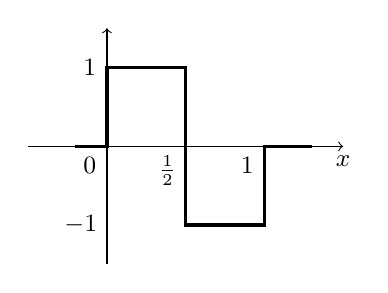
\begin{tikzpicture}[xscale=2]
      \draw [thin,->] (0,-1.5) -- (0,1.5);
      \draw [thin,->] (-0.5,0) -- (1.5,0) node[below]{\small$x$};
      \draw [very thick] (-0.2,0) -- (0,0) node[below left]{\small$0$} -- (0,1) node[left]{\small $1$} -- (0.5,1) -- (0.5,-1) -- (1,-1) -- (1,0) node[below left]{\small $1$} -- (1.3,0);
      \node at (0,-1)[left]{\small$-1$};
      \node at (0.5,0)[below left]{\small $\frac{1}{2}$};
    \end{tikzpicture}
    \caption{Haar mother wavelet $\psi(x)$}
    \label{fig:haar_mother}
  \end{subfigure}
  \caption{The scaling function and wavelet function for the Haar wavelets.}
  \label{fig:haar_1d}
\end{figure}

For example, for the \emph{Haar wavelets} the scaling function is given by
\begin{equation}
  \label{eqn:haar_scale}
  \phi(x) = \left\{ \begin{array}{rl}
    1& \qquad \mbox{if $0\leq x < 1$}\\
    0& \qquad \mbox{otherwise}
  \end{array}\right.
\end{equation}
See Figure \ref{fig:haar_scaling} for a plot of $\phi(x)$.

Given the scaling function $\phi(x)$, we can define the following basis for $V^j$:
\begin{equation}
  \label{eqn:haar_scaling_basis}
  \phi_k^j(x) := 2^{j/2}\phi(2^j x-k) \qquad k = 0,\cdots, 2^j-1
\end{equation}

Using this basis, we can decompose our signal $v(x)\in V^q$ as 
\begin{equation*}
  v(x) = \sum_{k=0}^{2^q-1} c_k^q \phi_k^q(x)
\end{equation*}
For the scaling function defined in equation (\ref{eqn:haar_scale}), we have that $c_k^q = v_{k+1}$.

To obtain \emph{wavelets}, consider the \emph{orthogonal complement} of $V^j$ in $V^{j+1}$ and denote it $W^j$. 
That is, $W^j = \{f \in V^{j+1} :\quad \langle f,g\rangle = 0\quad \forall g \in V^j\}$ where the inner product $\langle f,g\rangle$ is given by
\begin{equation*}
  \langle f,g\rangle = \int_0^1f(x)g(x)dx.
\end{equation*}
By forming a basis for $W^j$, we obtain a set of \emph{wavelet functions} $\{\psi_k^j,\, k=0,\cdots,2^j-1\}$.
Wavelet functions can be constructed by scaling and shifting a so-called \emph{mother wavelet} $\psi(x)$ as follows:
\begin{equation}
  \label{eqn:haar_wavelet_basis}
  \psi_k^j(x) = 2^{j/2}\psi(2^j x - k) \qquad k = 0,\cdots, 2^j-1
\end{equation}

For the Haar wavelets, the mother wavelet is given by:
\begin{equation}
\label{eqn:haar_mother}
  \psi(x) = \left\{\begin{array}{rl}
  1&\qquad 0 \leq x < 1/2\\
  -1&\qquad 1/2 \leq x < 1\\
  0&\qquad\mbox{otherwise}
  \end{array}\right.
\end{equation}
The Haar mother wavelet is shown in Figure \ref{fig:haar_mother}.

Note that, since the scaling functions $\phi_k^j$ form a basis of $V^j$ and the wavelet functions $\psi_k^j$ form a basis of $W^k$, and since $W^j$ is the orthogonal complement to $V^j$ in $V^{j+1}$, it follows that the set $\{\phi_k^j, \psi_k^j: k=0,\cdots,2^j-1\}$ forms a basis of the vector space $V^{j+1}$.

This allows us to express our signal $v \in V^q$ as 
\begin{equation*}
  v(x) = \sum_{k=0}^{2^{q-1}-1} d_k^{q-1}\psi_k^{q-1}(x) + \sum_{k=0}^{2^{q-1}-1} c_k^{q-1}\phi_k^{q-1}(x)
\end{equation*}
This gives us the first level of the discrete wavelet transform of $v$.
The coefficients $c_k$ and $d_k$ are sometimes referred to as ``approximation'' coefficients and ``detail'' coefficients, respectively.

We can continue the decomposition by splitting the basis for $V^{q-1}$ into the bases for $V^{q-2}$ and $W^{q-2}$ to get the next level of the transform:
\begin{equation*}
  v(x) = \sum_{k=0}^{2^{q-1}-1} d_k^{q-1}\psi_k^{q-1}(x) + \sum_{k=0}^{2^{q-2}-1} d_k^{q-2}\psi_k^{q-2}(x) + \sum_{k=0}^{2^{q-2}-1} c_k^{q-2}\phi_k^{q-2}(x)
\end{equation*}
To get the full decomposition, we continue in this fashion up to the $q$th level:
\begin{equation*}
  v(x) = \sum_{j=0}^{q-1} \sum_{k=0}^{2^j-1} d_k^{j} \psi_k^j(x) + c_0^0\phi(x)
\end{equation*}
The full DWT of $\bm v$ consists of the coefficients $\{c_0^0, d_k^j:\,j=0,\cdots,q-1, \, k=0,\cdots,2^j-1\}$.


\subsection{Computing the DWT}

\begin{figure}
  \centering
  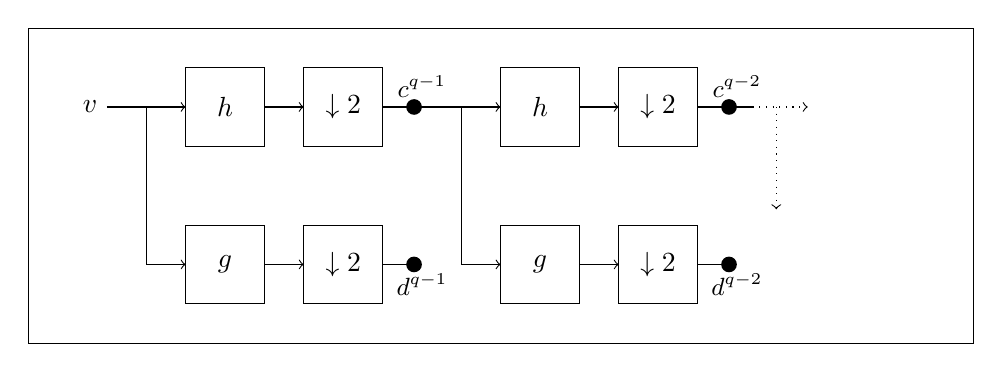
\begin{tikzpicture}
    \draw (0,0) rectangle (12,4);
    \draw (1,3) node[left]{$v$} -- (1.5,3);
    \draw (1.5,1) -- (1.5,3);
    \draw [->](1.5,3) -- (2,3);
    \draw [->](1.5,1) -- (2,1);
    \draw (2,2.5) rectangle (3,3.5);
    \node at (2.5,3) {$h$};
    \draw (2,0.5) rectangle (3,1.5);
    \node at (2.5,1) {$g$};
    \draw [->](3,1) -- (3.5,1);
    \draw (3.5,0.5) rectangle (4.5,1.5);
    \node at (4,1) {$\downarrow 2$};
    \draw (4.5,1) -- (5,1) node [below] {\small$d^{q-1}$};
    \node at (4.9,1)[shape=circle, fill=black, inner sep=2pt, minimum size=2pt] {};
    \draw [->](3,3) -- (3.5,3);
    \draw (3.5,2.5) rectangle (4.5,3.5);
    \node at (4,3) {$\downarrow 2$};
    \draw [->](4.5,3) -- (6,3);
    \draw [->](5.5,3) -- (5.5,1) -- (6,1);
    \node at (5,3) [above] {\small$c^{q-1}$};
    \node at (4.9,3) [shape=circle, fill=black, inner sep=2pt, minimum size=2pt] {};
    \draw (6,2.5) rectangle (7,3.5);
    \node at (6.5,3){$h$};
    \draw (6,0.5) rectangle (7,1.5);    
    \node at (6.5,1){$g$};
    \draw [->] (7,3) -- (7.5,3);
    \draw (7.5,2.5) rectangle (8.5,3.5);
    \node at (8,3) {$\downarrow 2$};
    \draw [->] (7,1) -- (7.5,1);
    \draw (7.5,0.5) rectangle (8.5,1.5);
    \node at (8,1) {$\downarrow 2$};
    \draw (8.5,1) -- (9,1) node [below] {\small$d^{q-2}$};
    \node at (8.9,1) [shape=circle, fill=black, inner sep=2pt, minimum size=2pt] {};
    \draw (8.5,3) -- (9.2,3);
    \draw [->,dotted](9.2,3) -- (9.9,3);
    \draw [->,dotted](9.5,3) -- (9.5,1.7);
    \node at (8.9,3) [shape=circle, fill=black, inner sep=2pt, minimum size=2pt] {};
    \node at (9,3) [above] {\small$c^{q-2}$};
  \end{tikzpicture}
  \caption[Filter Bank computation of the DWT]{The first two levels of the DWT of the signal $\bm v$ of length $2^q$ via a filter bank.}
  \label{fig:filterbank}
\end{figure}

In practice, we can compute one level of the DWT coefficients by passing the signal $v$ through a \emph{low-pass filter} $h$ and a high-pass filter $g$, respectively, and then downsampling the results by a factor of two.
Passing $v$ through the filters $h$ and $g$ results in the \emph{convolutions}:
\begin{equation*}
  \begin{split}
    (v\star h)(x) &= \sum_{k=-\infty}^\infty v(k)h(x-k)\\
    (v\star g)(x) &= \sum_{k=-\infty}^\infty v(k)g(x-k)
  \end{split}
\end{equation*}
To downsample by a factor of two, we remove every second sample:
\begin{equation*}
  (v\downarrow 2)(x) := v(2x)
\end{equation*}

Overall, these computations can be done by multiplying the vector $\bm v$ by a matrix $\bm H$ and a matrix $\bm G$ to get the approximation and detail coefficients, repectively.

To compute the next level, we take the approximation coefficients of the current stage and pass them again through the filter bank.
The procedure is depicted in Figure \ref{fig:filterbank}.

The coefficients of the filters $h(x)$ and $g(x)$ depend on our choice of the scaling function $\phi(x)$ and mother wavelet function $\psi(x)$.
They satisfy the following relations:
\begin{equation*}
  \begin{split}
    \phi(x) &= \sqrt{2}\sum_{k=-\infty}^\infty h(k)\phi(2x - k)\\
    \psi(x) &= \sqrt{2}\sum_{k=-\infty}^\infty g(k)\phi(2x - k)
  \end{split}
\end{equation*}
as well as
\begin{equation*}
  g(k) = (-1)^k h(1-k).
\end{equation*}

For the Haar wavelets (\ref{eqn:haar_scale},\ref{eqn:haar_mother}), the filter coefficients are
\begin{equation*}
  \begin{split}
    h(0) = h(1) &= \frac{1}{\sqrt{2}}, \qquad h(k) = 0 \mbox{  if $k\neq 0,1$}\\
    g(0) = -g(1) &= \frac{1}{\sqrt{2}}, \qquad g(k) = 0 \mbox{  if $k\neq 0,1$}
  \end{split}
\end{equation*}

The first level approximation coefficients of the Haar DWT of signal $\bm v \in\mathbb{R}^M$, with $M=2^q$, are thus given by $\bm H^q \bm v$ where $\bm H^q$ is the $2^{q-1}\times 2^q$ matrix given by
\begin{equation}
  \label{eqn:haar_H}
  \bm H^q_{haar} = \frac{1}{\sqrt{2}} \begin{bmatrix}
    1&1&0&0&\cdots&0&0\\
    0&0&1&1&\cdots&0&0\\
    \vdots&\vdots&\vdots&\vdots&\ddots&\vdots&\vdots\\
    0&0&0&0&\cdots&1&1
  \end{bmatrix}
\end{equation}
To get the corresponding detail coefficients, we multiply $\bm v$ by the $2^{q-1}\times 2^q$ matrix $\bm G^q$ given by
\begin{equation}
  \label{eqn:haar_G}
  \bm G^q_{haar} = \frac{1}{\sqrt{2}} \begin{bmatrix}
    1&-1&0&0&\cdots&0&0\\
    0&0&1&-1&\cdots&0&0\\
    \vdots&\vdots&\vdots&\vdots&\ddots&\vdots&\vdots\\
    0&0&0&0&\cdots&1&-1
  \end{bmatrix}
\end{equation}

Overall to perform the discrete Haar wavelet transform at the first scale, we multiply $\bm v$ by
\begin{equation*}
  \bm P^{(1)}_{haar} = \begin{bmatrix}
    \bm H^q \\
    \bm G^q \\
  \end{bmatrix}
\end{equation*}
where we dropped $haar$-subscript on $\bm H$ and $\bm G$ for ease of viewing.

To compute the transform at the second scale, we replace $\bm H^q$ by $\bm H^{q-1}\bm H^q$ and $\bm G^{q-1}\bm h^q$:
\begin{equation*}
  \bm P^{(2)}_{haar} = \begin{bmatrix}
    \bm H^{q-1} \bm H^q \\
    \bm G^{q-1} \bm H^q \\
    \bm G^q \\
  \end{bmatrix}
\end{equation*}

We can continue this process until the $q$th scale to get the full Haar wavelet transform matrix:
\begin{equation*}
  \bm P^{(q)}_{haar} = \begin{bmatrix}
    \bm H^1 \bm H^2 \cdots \bm H^{q-1} \bm H^q \\
    \bm G^1 \bm H^2 \cdots \bm H^{q-1} \bm H^q \\
    \vdots\\
    \bm G^{q-2} \bm H^{q-1} \bm H^q \\
    \bm G^{q-1} \bm H^q \\
    \bm G^q \\
  \end{bmatrix}
\end{equation*}

To form the basis matrix $\bm\Psi$ such that $\bm v = \bm\Psi\bm w$ corresponding to the stage $j$ DWT, we can invert the matrix $\bm P^{(j)}_{haar}$:
\begin{equation}
  \label{eqn:dwt_basis}
  \bm\Psi = \left(\bm P^{(j)}_{haar}\right)^{-1}
\end{equation}
In practice, one usually works with wavelet functions that lead to orthogonal transform matrices, so that $\left(\bm P^{(j)}\right)^{-1}=\left(\bm P^{(j)}\right)^T$.
The Haar wavelets satisfy this orthoganility condition.
Therefore, the basis matrix $\bm\Psi$ from equation (\ref{eqn:dwt_basis}) can also be obtained as follows:
\begin{equation}
  \label{eqn:haar1_basis}
  \bm\Psi = \left(\bm P^{(j)}_{haar}\right)^T.
\end{equation}

[CAVEAT boundary conditions]

\subsection{Two-Dimensional Haar Wavelets}
In Figure \ref{fig:haar_1d}, we showed the 1-dimensional Haar scaling function $\phi(x)$ and wavelet function $\psi(x)$.
In general, we can define the 2-dimensional scaling wavelet functions by taking the products of their one-dimensional versions:
\begin{equation}
\label{eqn:2d_haar_wavelets}
  \begin{split}
    \phi(x,y) &= \phi(x) \phi(y)\\
    \psi^H(x,y) &= \phi(x) \psi(y) \\
    \psi^V(x,y) &= \psi(x) \phi(y) \\
    \psi^D(x,y) &= \psi(x) \psi(y)
  \end{split}
\end{equation}

\begin{figure}
\centering
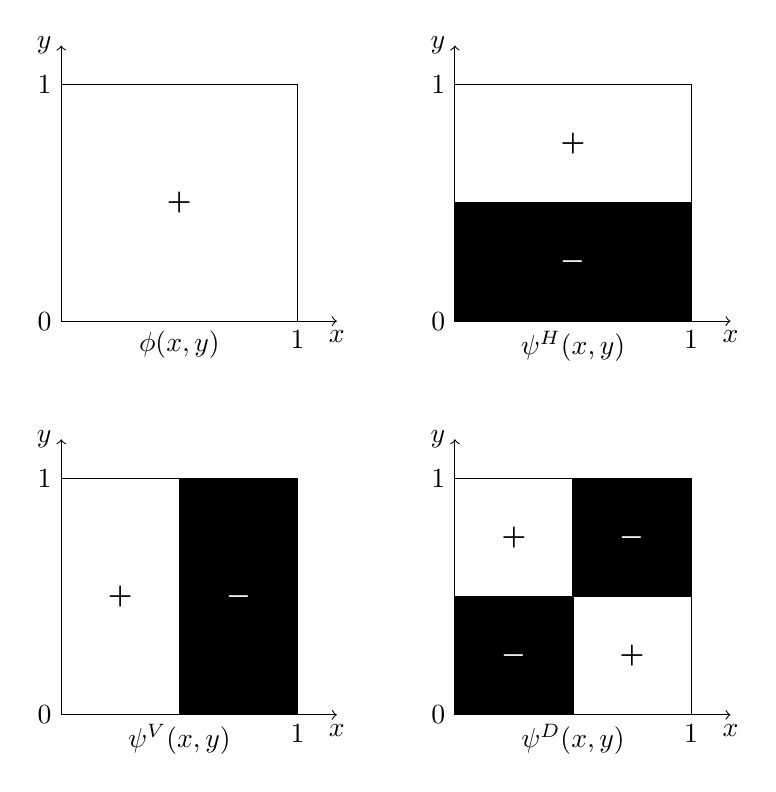
\begin{tikzpicture}
  \draw (0,5) rectangle (3,8);
  \draw (5,5) rectangle (8,8);
  \draw (0,0) rectangle (3,3);
  \draw (5,0) rectangle (8,3);

  \draw [<->] (0,8.5) -- (0,5) -- (3.5,5);
  \draw [<->] (5,8.5) -- (5,5) -- (8.5,5);
  \draw [<->] (0,3.5) -- (0,0) -- (3.5,0);
  \draw [<->] (5,3.5) -- (5,0) -- (8.5,0);

  \node at (1.5,5) [below] {$\phi(x,y)$};
  \node at (0,5) [left] {$0$};
  \node at (0,8) [left] {$1$};
  \node at (3,5) [below] {$1$};
  \node at (3.5,5) [below] {$x$};
  \node at (0,8.5) [left] {$y$};

  \node at (6.5,5) [below] {$\psi^H(x,y)$};
  \node at (5,5) [left] {$0$};
  \node at (5,8) [left] {$1$};
  \node at (8,5) [below] {$1$};
  \node at (8.5,5) [below] {$x$};
  \node at (5,8.5) [left] {$y$};

  \node at (1.5,0) [below] {$\psi^V(x,y)$};
  \node at (0,0) [left] {$0$};
  \node at (0,3) [left] {$1$};
  \node at (3,0) [below] {$1$};
  \node at (3.5,0) [below] {$x$};
  \node at (0,3.5) [left] {$y$};

  \node at (6.5,0) [below] {$\psi^D(x,y)$};
  \node at (5,0) [left] {$0$};
  \node at (5,3) [left] {$1$};
  \node at (8,0) [below] {$1$};
  \node at (8.5,0) [below] {$x$};
  \node at (5,3.5) [left] {$y$};

  \draw [fill=black] (5,5) rectangle (8,6.5);
  \draw [fill=black] (1.5,0) rectangle (3,3);
  \draw [fill=black] (5,0) rectangle (6.5,1.5);
  \draw [fill=black] (6.5,1.5) rectangle (8,3);

  \node at (1.5,6.5){$\bm +$};  

  \node at (6.5,7.25){$\bm +$};
  \node at (6.5,5.75){\textcolor{white}{$\bm -$}};

  \node at (0.75,1.5){$\bm +$};
  \node at (2.25,1.5){\textcolor{white}{$\bm -$}};

  \node at (5.75,2.25){$\bm +$};
  \node at (7.25,0.75){$\bm +$};
  \node at (5.75,0.75){\textcolor{white}{$\bm -$}};
  \node at (7.25,2.25){\textcolor{white}{$\bm -$}};
\end{tikzpicture}
\caption[2-D Haar Wavelets]{The 2-D Haar scaling function and wavelet functions.
  Inside the $[0,1]\times [0,1]$ square, white corresponds to $+2$ and black corresponds to $-1$. 
  The functions are zero outside the unit square.}
\label{fig:haar_2d}
\end{figure}

Where the superscripts $H,V$ and $D$ refer to the high-pass filters in the horizontal, vertical and diagonal direction, respectively.
These functions are illustrated in Figure \ref{fig:haar_2d} for the Haar wavelet system.
The 2-D Haar wavelet functions act as \emph{edge detectors} in their respective directions.
For example, if we pass a $2\times 2$ image patch through the $\psi^V$ filter, the corresponding detail coefficient will be small unless there is sharp change in pixel intensities between the left side and right side of the patch, i.e. unless there is a vertical edge.

\begin{figure}
\centering
\begin{subfigure}{0.4\textwidth}
  \includegraphics[width=\textwidth]{Chapter3/Images/haar2_scale1.png}
  \caption{Scale 1}
\end{subfigure}
\begin{subfigure}{0.4\textwidth}
  \includegraphics[width=\textwidth]{Chapter3/Images/haar2_scale2.png}
  \caption{Scale 2}
\end{subfigure}
\caption[2-D Haar basis functions]{The haar basis functions at the first scale (a) and the second scale (b). The DWT would use these basis functions to decompose a $4\times 4$ image.}
\label{fig:haar2_basis}
\end{figure}

\begin{figure}
\centering
\begin{subfigure}{0.4\textwidth}
  \includegraphics[width=\textwidth]{Chapter3/Images/house.png}
  \caption{Original $512\times 512$ image}
\end{subfigure}
\begin{subfigure}{0.4\textwidth}
  \includegraphics[width=\textwidth]{Chapter3/Images/dwt1.png}
  \caption{Scale 1 DWT}
\end{subfigure}
\begin{subfigure}{0.4\textwidth}
  \includegraphics[width=\textwidth]{Chapter3/Images/dwt2.png}
  \caption{Scale 2 DWT}
\end{subfigure}
\begin{subfigure}{0.4\textwidth}
  \includegraphics[width=\textwidth]{Chapter3/Images/dwt9.png}
  \caption{Scale 9 DWT}
\end{subfigure}
\caption[2-D Haar DWT Example]{The 2-D DWT using Haar wavelets of a digital image (a) of size $512\times 512$.
  We compute the DWT at the first and the second scale (b,c) as well as the full DWT (d).
  In (d), we have a single approximation coefficient at the top left corner.
  In (b,c,d), the brightness of a pixel increases monotonically with the size of the corresponding DWT coefficient.
  We have enhanced the detail coefficients (relative to the approximation coefficients) for better visibility.}
\label{fig:dwt2}
\end{figure}

The wavelet basis functions for scale $j$ can be formed in two different ways.
In the so-called ``standard'' construction \cite{stollnitz1995}, we first compute the DWT for scale $j$ for each column, followed by computing the scale-$J$ DWT on the intermediate result for each row.

The non-standard construction, on the other hand, builds up the scale-$j$ iteratively transforming the columns and the rows.
First, we perform the standard construction, but only for the first scale.
%First, we compute the level-1 DWT for each column, followed by the level-1 DWT for each row. 
Next, we do another level-1 DWT, but only on the approximation coefficients of the previous stage.
We repeat this process $j$ times to get the level-$j$ DWT.

In this document, we will only consider the non-standard construction of the DWT basis.
The reason is that the basis functions resulting from the non-standard construction always have square support and to keep in line with \cite{pilikos2014}.

In Figure \ref{fig:haar2_basis}, we illustrate the basis functions resulting from the non-standard construction. 
We show two sets of basis functions that can be used by the Haar DWT to decompose a signal of size $4\times 4$, one corresponding to the first scale and another set corresponding to the level 2 decomposition.
The DWT of a digital image is illustrated at various levels in Figure \ref{fig:dwt2}.
One can clearly see that the high-pass filters corresponding to the Haar wavelets act as edge detectors.


\section{Basis Matrix for 2-D and 3-D Signals}
So far, we have displayed two-dimensional signals as matrices and three-dimensional signals as 3-D arrays (also known as ``3-D matrices'', third-order tensors, or ``cubes'').
To reconcile this with the notation used in Chapter \ref{ch:cs}, we need to \emph{vectorize} the multi-dimensional signal $\bm v$.
More importantly, the RVM in Chapter \ref{ch:rvm} is agnostic of the dimensionality of the signal. 
It takes as input a target vector $\bm y$ and a design matrix $\bm \Phi$ and outputs a weights vector $\bm w$.
Any information about the structur of a signal (such as its dimensionality) is encoded in the design matrix.
Therefore, it is important that we vectorize our multi-dimensional signals and also form the basis matrix $\bm Psi$ from the transform matrices (corresponding to the DCT/DWT/etc) in a way that is consistent with the vectorization.

We will define the particular vectorization scheme that was used in our algorithm and describe how we built the basis matrices from the specific (inverse) transform matrices.

\subsection{Basis Matrix for One-Dimensional Signals}
We start with 1-D signals. 
This case is trivial, since a one-dimensional signal $\bm v$ can directly be treated as a vector in $\mathbb{R}^M$, where $M$ is the length of the signal.

The basis matrix matrix, in this case, is simply the inverse transform matrix.
So, for the DCT, the basis matrix is $\bm\Psi = \bm P$, where $\bm P$ is defined in equation (\ref{eqn:idct_basis}).
We have defined the basis matrix corresponding to the discrete Haar wavelet transform in equation (\ref{eqn:haar1_basis}).

\subsection{Basis Matrix for Two-Dimensional Signals}
\label{sect:vectorize2d}
Suppose $\bm v$ is a two-dimensional signal of size $r\times c$ (i.e. $r$ rows and $c$ columns).
Suppose further that $r$ and $c$ are powers of 2, $r=2^{q_1}$ and $c = 2^{q_2}$, say.

We vectorize $\bm v$ in a row-major fashion.
To be explicit, let $\bm v_j^T$ be the $j$th row of $\bm v\in\mathbb{R}^{r\times c}$.
The vectorized form of $\bm v$ is then given by
\begin{equation*}
  \bm v^V = \begin{bmatrix}
    \bm v_1 \\
    \bm v_2 \\
    \vdots \\
    \bm v_r
  \end{bmatrix}
\end{equation*}
where we use the $V$ superscript to indicate the vectorized signal.
Thus, we end up with a long vector $\bm v^V \in \mathbb{R}^{rc}$.

To form the basis matrix corresponding to the two-dimensional DCT, we use the DCT's seperability property.
Let $\bm\Psi_r$ and $\bm\Psi_c$ be the DCT basis matrices corresponding to one-dimensional signals of length $r$ and $c$, respectively.
The basis matrix corresponding to $\bm v^V$ is then given by forming the \emph{kronecker product} of $\bm\Psi_c$ and $\bm\Psi_r$:
\begin{equation*}
\label{eqn:dct3_basis}
  \bm\Psi = \bm\Psi_c \otimes \bm\Psi_r
\end{equation*}
The kronecker product $P \otimes Q$ between matrices $P$ and $Q$ with dimensions $m_P \times n_P$ and $m_Q \times n_Q$, respectively,  is defined to be the block matrix
\begin{equation}
\label{eqn:kron}
\begin{bmatrix}
P_{1,1} Q & P_{1,2} Q & \cdots & P_{1,n_P} Q \\
P_{2,1} Q & P_{2,2} Q & \cdots & P_{2,n_P} Q \\
\vdots&\vdots&\ddots&\vdots \\
P_{m_P,1} Q & P_{m_P,2} Q & \cdots & P_{m_P,n_P} Q \\
\end{bmatrix}
\end{equation}
of size $(m_Pm_Q) \times (n_Pn_Q)$.

For the 2-D Haar DWT at the first scale, the basis matrix is constructed in a similar fashion.
Let $\bm H^{q_1}$ and $\bm H^{q_2}$ be defined according to equation (\ref{eqn:haar_H}), and let $\bm G^{q_1}$ and $\bm G^{q_2}$  be formed according to (\ref{eqn:haar_G}) (where we dropped the $haar$ subscript. 
The basis matrix is constructed as follows:
\begin{equation*}
  \bm \Psi = 
  \begin{bmatrix}
    \bm H^{q_2} \otimes\bm H^{q_1} \\
    \bm H^{q_2} \otimes \bm G^{q_1} \\
    \bm G^{q_2} \otimes \bm H^{q_1} \\
    \bm G^{q_2} \otimes \bm G^{q_1} 
  \end{bmatrix}^T.
\end{equation*}
For a signal of size $2^{q_1}\times 2^{q_2}$, we can build a cascade up to the $q$th scale, where $q = \min\{q_1,q_2\}$.
The resulting basis matrix is given by
\begin{equation*}
\label{eqn:haar2_fullbasis}
  \bm \Psi = 
  \begin{bmatrix}
    (\bm H^{q_2-q}\bm H^{q_2-q+1} \cdots \bm H^{q_2}) \otimes (\bm H^{q_1-q} \bm H^{q_1-q+1}\cdots\bm H^{q_1}) \\
    (\bm H^{q_2-q}\bm H^{q_2-q+1} \cdots \bm H^{q_2}) \otimes (\bm G^{q_1-q} \bm H^{q_1-q+1}\cdots\bm H^{q_1}) \\
    (\bm G^{q_2-q}\bm H^{q_2-q+1} \cdots \bm H^{q_2}) \otimes (\bm H^{q_1-q} \bm H^{q_1-q+1}\cdots\bm H^{q_1}) \\
    (\bm G^{q_2-q}\bm H^{q_2-q+1} \cdots \bm H^{q_2}) \otimes (\bm G^{q_1-q} \bm H^{q_1-q+1}\cdots\bm H^{q_1}) \\
    (\bm H^{q_2-q+1}\bm H^{q_2-q+2} \cdots \bm H^{q_2}) \otimes (\bm G^{q_1-q+1} \bm H^{q_1-q+2}\cdots\bm H^{q_1}) \\
    (\bm G^{q_2-q+1}\bm H^{q_2-q+2} \cdots \bm H^{q_2}) \otimes (\bm H^{q_1-q+1} \bm H^{q_1-q+2}\cdots\bm H^{q_1}) \\
    (\bm G^{q_2-q+1}\bm H^{q_2-q+2} \cdots \bm H^{q_2}) \otimes (\bm G^{q_1-q+1} \bm H^{q_1-q+2}\cdots\bm H^{q_1}) \\
    \vdots \\
    (\bm G^{q_2-2}\bm H^{q_2-1} \bm H^{q_2}) \otimes (\bm G^{q_1-2}\bm H^{q_1-1}\bm H^{q_1}) \\
    (\bm H^{q_2-1} \bm H^{q_2}) \otimes (\bm G^{q_1-1}\bm H^{q_1}) \\
    (\bm G^{q_2-1} \bm H^{q_2}) \otimes (\bm H^{q_1-1}\bm H^{q_1}) \\
    (\bm G^{q_2-1} \bm H^{q_2}) \otimes (\bm G^{q_1-1}\bm H^{q_1}) \\
    \bm H^{q_2} \otimes \bm G^{q_1} \\
    \bm G^{q_2} \otimes \bm H^{q_1} \\
    \bm G^{q_2} \otimes \bm G^{q_1} 
  \end{bmatrix}^T.
\end{equation*}
Note that the dimensions of the basis matrix are $(rc)\times (rc)$, regardless of the scale that we use.

% Like the DCT, the DWT also has the \emph{seperability} property.
% Thus, to perform the DWT on a two-dimensional signal, such as an image, we first compute the 1-D DWT for each column.
% Next, we compute the 1-D DWT on each row of the preceding result.
% Note that, due to multi-resolution properties of the DWT, we have a choice on how we compute the 2-D DWT.
% We could either perform the full decomposition (up to the highest possible scale) on the first dimension, followed by 
% For the Haar wavelets, it can be easily verified that 
% \begin{equation*}
%   \langle\psi_k^p,\psi_l^q\rangle = 
%   \left\{\begin{array}{rl}
%       1&\qquad\mbox{if $k=l$ and $p=q$}\\
%       0&\qquad\mbox{otherwise}
%     \end{array}
%   \right.
% \end{equation*}
% We also know that 
% \begin{equation*}
%   \langle\phi_k^j,\psi_l^j\rangle = 0\qquad \forall k,l,j
% \end{equation*}
% since the sets $\{\psi^j_k, k = 0,\cdots,2^j-1\}$ and $\{\phi^j_k, k = 0,\cdots,2^j-1\}$ each span a space that are orthogonal complements to each other.



% For a deeper introduction into wavelets see \cite{stollnitz1995}.
% For more information on wavelet compression techniques, see \cite{devore1992}.





\include{chapter}

\chapter{Bayesian Compressive Sensing}
\label{ch:bcs}
In this chapter, we combine the Compressive Sensing framework from Chapter \ref{ch:cs} with the Bayesian framework from Chapter \ref{ch:rvm}.



% In order to reconstruct the image, we use the estimated posterior mean to ``predict'' what a pixel value $y^*$ should be at a location $x^*$ in which information was missing:
% \begin{equation}
% y^* = \bs w^T\bs\psi(x^*)
% \end{equation}

% \begin{figure}
% \center
% \includegraphics{Images/0.png}
% \includegraphics{Images/3.png}
% \caption{Corrupted signal $\bs y$ (left) and reconstructed signal $\hat{\bs x}$ (right) using a cascade of 3 RVMs with Haar basis functions (see \cite{pilikos2014}).}
% \label{fig:lennareconstruction}
% \end{figure}

% Apart from achieving sparse solutions, one further desirable feature of the RVM is that the model provides error bars for its predictions.
% This is used in \cite{pilikos2014} to construct a multi-scale cascade of RVM estimations and achieve significant performance boosts.

% An example of this can be seen in Figure \ref{fig:lennareconstruction}.



\chapter{Implementation Details and Code optimization}
\label{ch:code}

Talk about code relevant to previous chapter.

Code specific for results goes in the results chapter,

\begin{enumerate}
\item Blocks
\item Parallelization
\item Short FastRVM
\item Modified Error Bars
\end{enumerate}


\chapter{Results}
\label{ch:results}
\begin{enumerate}
\item Metrics: PSNR, (Relative Error), (FSIM)
\item DCT for BCS of images and videos (put in Results)?
\item Full Res vs Pre-compressed: With full res, I need a lot of samples to get perfect reconstruction. With pre-comp, I'm not sure.
\item Curve: Performance vs Compression
\item Masks vs Gaussian vs Rademacher
\item Full Scale Haar vs DCT
\item What't the best performance I can achieve? How does it compare to the lit?
\item Example Results
\item MSCE was done to solve the signal interpolation. In particular, to fix the problem with small support of wavelets while still using their power.
\item Problem: Slow. Solution: Parallelization.
\item Problem: Limited to signal interpolation. Solution: Use CS sensing matrices (but Cascade don't work yet).
\item Do we even need the cascade? What if we jump straight to the third scale.
\item Can we improve the performance of the interpolator? 
\item Small blocks reduce performance due to less data for RVM
\item When is MPI useful
\item What should $\sigma^2$ be.
\item Modified Error Bars
\end{enumerate}

\section{Video Reconstruction for General Sensing Matrices}
\begin{enumerate}
\item For certain basis functions, the matrix $\bm\Psi$ will be very sparse. It is possible to exploit this sparsity to significantly reduce the memory requirements. 
\item General sensing Matrix for BCS of videos?
\end{enumerate}


\chapter{Conclusion}
\label{ch:conclusion}

For the MPhil thesis, we set out to develop a generic Compressive Sensing algorithm that provides high quality reconstructions of video signals from relatively small numbers of samples.


In this thesis, we investigated the efficacy of the Bayesian Compressive Sensing framework for efficient reconstruction of highly under-sampled video signals.
We developed an extension to the Multi-Scale Cascade of Estimations algorithm that achieves near-perfect reconstructions of videos from a very small set of measurements.

To do so, we constructed three-dimensional wavelet basis functions that allow for a highly compressible representation of the video signal.
Compressive Sensing inversion is then formulated as a machine learning problem and the Relevance Vector Machine was employed to find highly sparse solutions.
To boost performance, a cascade of RVMs it built that exploits the multi-resolution properties of wavelet basis functions.

In order to deal with the large memory requirements of the algorithm, the reconstruction is performed in blockwise fashion.
We have also implemented the method as a distributed program, resulting in dramatically reduced execution times.

Future research could improve performance by extending these methods in various ways.
In order to fully harness the power of the MSCE for video interpolation, the implentation should be extended to accommodate different kinds of wavelets.
Using the simple Haar wavelets, the MSCE struggles to outperform a BCT that uses DCT basis functions.
It only shows its advantage in extremely undersampled situations ($N < 0.2M$).
Alternative sets of waveles, such as the CDF-9/7 wavelet that is used by the JPEG2000 format, may lead to sparser representations of the video signals. 

Furthermore, the speed of the algorithm can be increased by using a multi-threaded implementation of the Sequential Sparse Bayesian Learning Algorithm. 

Development of Bayesian approaches to Compressive Sensing systems is an active area of research.




%\setboolean{@twoside}{false}
%\includepdf[pages={1},angle=270]{gantt.pdf}
%\section*{Acknowledgements}
%Here I acknowledge the assistance of my supervisor, my industrial sponsor,
%and the effects of caffeine on my ability to produce this report on time.

%% The Appendices part is started with the command \appendix;
%% appendix sections are then done as normal sections
%\appendix

%% References
%%
%% Following citation commands can be used in the body text:
%% Usage of \cite is as follows:
%%   \cite{key}         ==>>  [#]
%%   \cite[chap. 2]{key} ==>> [#, chap. 2]
%%

%% References with bibTeX database:
%\section*{Bibliography}
\bibliographystyle{elsarticle-num}
%\bibliographystyle{apa}
\bibliography{referencesRVM.bib}

%% Authors are advised to submit their bibtex database files. They are
%% requested to list a bibtex style file in the manuscript if they do
%% not want to use elsarticle-num.bst.

%% References without bibTeX database:

% \begin{thebibliography}{00}

%% \bibitem must have the following form:
%%   \bibitem{key}...
%%

% \bibitem{}

% \end{thebibliography}


\end{document}

%%
%% End of file `rvm.tex'.